\section{核心技术路线与关键决策}
\label{sec:methodology}

本项目的技术路线最终收敛为一条比较清楚的主线：视觉负责动作阶段和
外部姿态，肌电负责目标肌和代偿肌的激活变化，FSM 负责确定性计数，
CompensationGRU 负责一段动作窗口内的质量判断，DeepSeek 和后台记录接口
负责交互与长期材料沉淀。本章按"感知—判断—交互"三层组织：先讲系统
怎么拿到稳定的视觉姿态与肌电特征，再讲怎么把它们转化为可判断的动作
质量，最后讲判断结果如何变成用户能感知、系统能记住的反馈。

\subsection{感知层：拿到能用的姿态与肌电}

本节说明系统如何同时拿到稳定的视觉姿态与肌电信号，以及为什么把视觉做成
本地与云端双路、把肌电做 MVC 归一化。

\subsubsection{视觉双路：本地 NPU 与云端 RTMPose}

视觉模块保留两条路线：本地 YOLOv5-Pose RKNN 路线和云端 RTMPose 路线。
YOLOv5 是 Ultralytics 维护的单阶段目标检测模型 \cite{yolov5}；
YOLOv5-Pose 由 Maji 等人在 YOLO-Pose 工作中提出，把人体关键点回归与
目标检测做成端到端单阶段输出 \cite{yolopose2022}，便于转换为 RKNN
后在 RK3399ProX 的 NPU 上运行。本地路线的意义是让系统在网络条件变化
时仍能获得骨架关键点，并把关节角度和动作阶段持续送入后续状态机。

RTMPose 是 OpenMMLab 团队提出、在 MMPose 工具箱中开源的实时人体姿态
估计模型 \cite{rtmpose,mmpose}。与 YOLOv5-Pose 的端到端单阶段不同，
RTMPose 走自顶向下的两阶段路线（先检测人体框，再回归关键点），
关键点精度通常更高但计算量更大，因此在系统中作为云端 GPU 备选路线：
板端把摄像头帧发到云端服务，云端返回关键点 JSON，板端再把结果写入
统一姿态状态。

两条路线通过 \code{/dev/shm/vision_mode.json} 切换，最终都输出到统一的
姿态数据接口。这样的设计不是简单堆叠模型，而是保留探索空间：本地 NPU
路线关注低依赖运行，云端 RTMPose 路线关注关键点质量，两者服务于同一套
FSM、GRU 和训练反馈链路。

\begin{figure}[htbp]
    \centering
    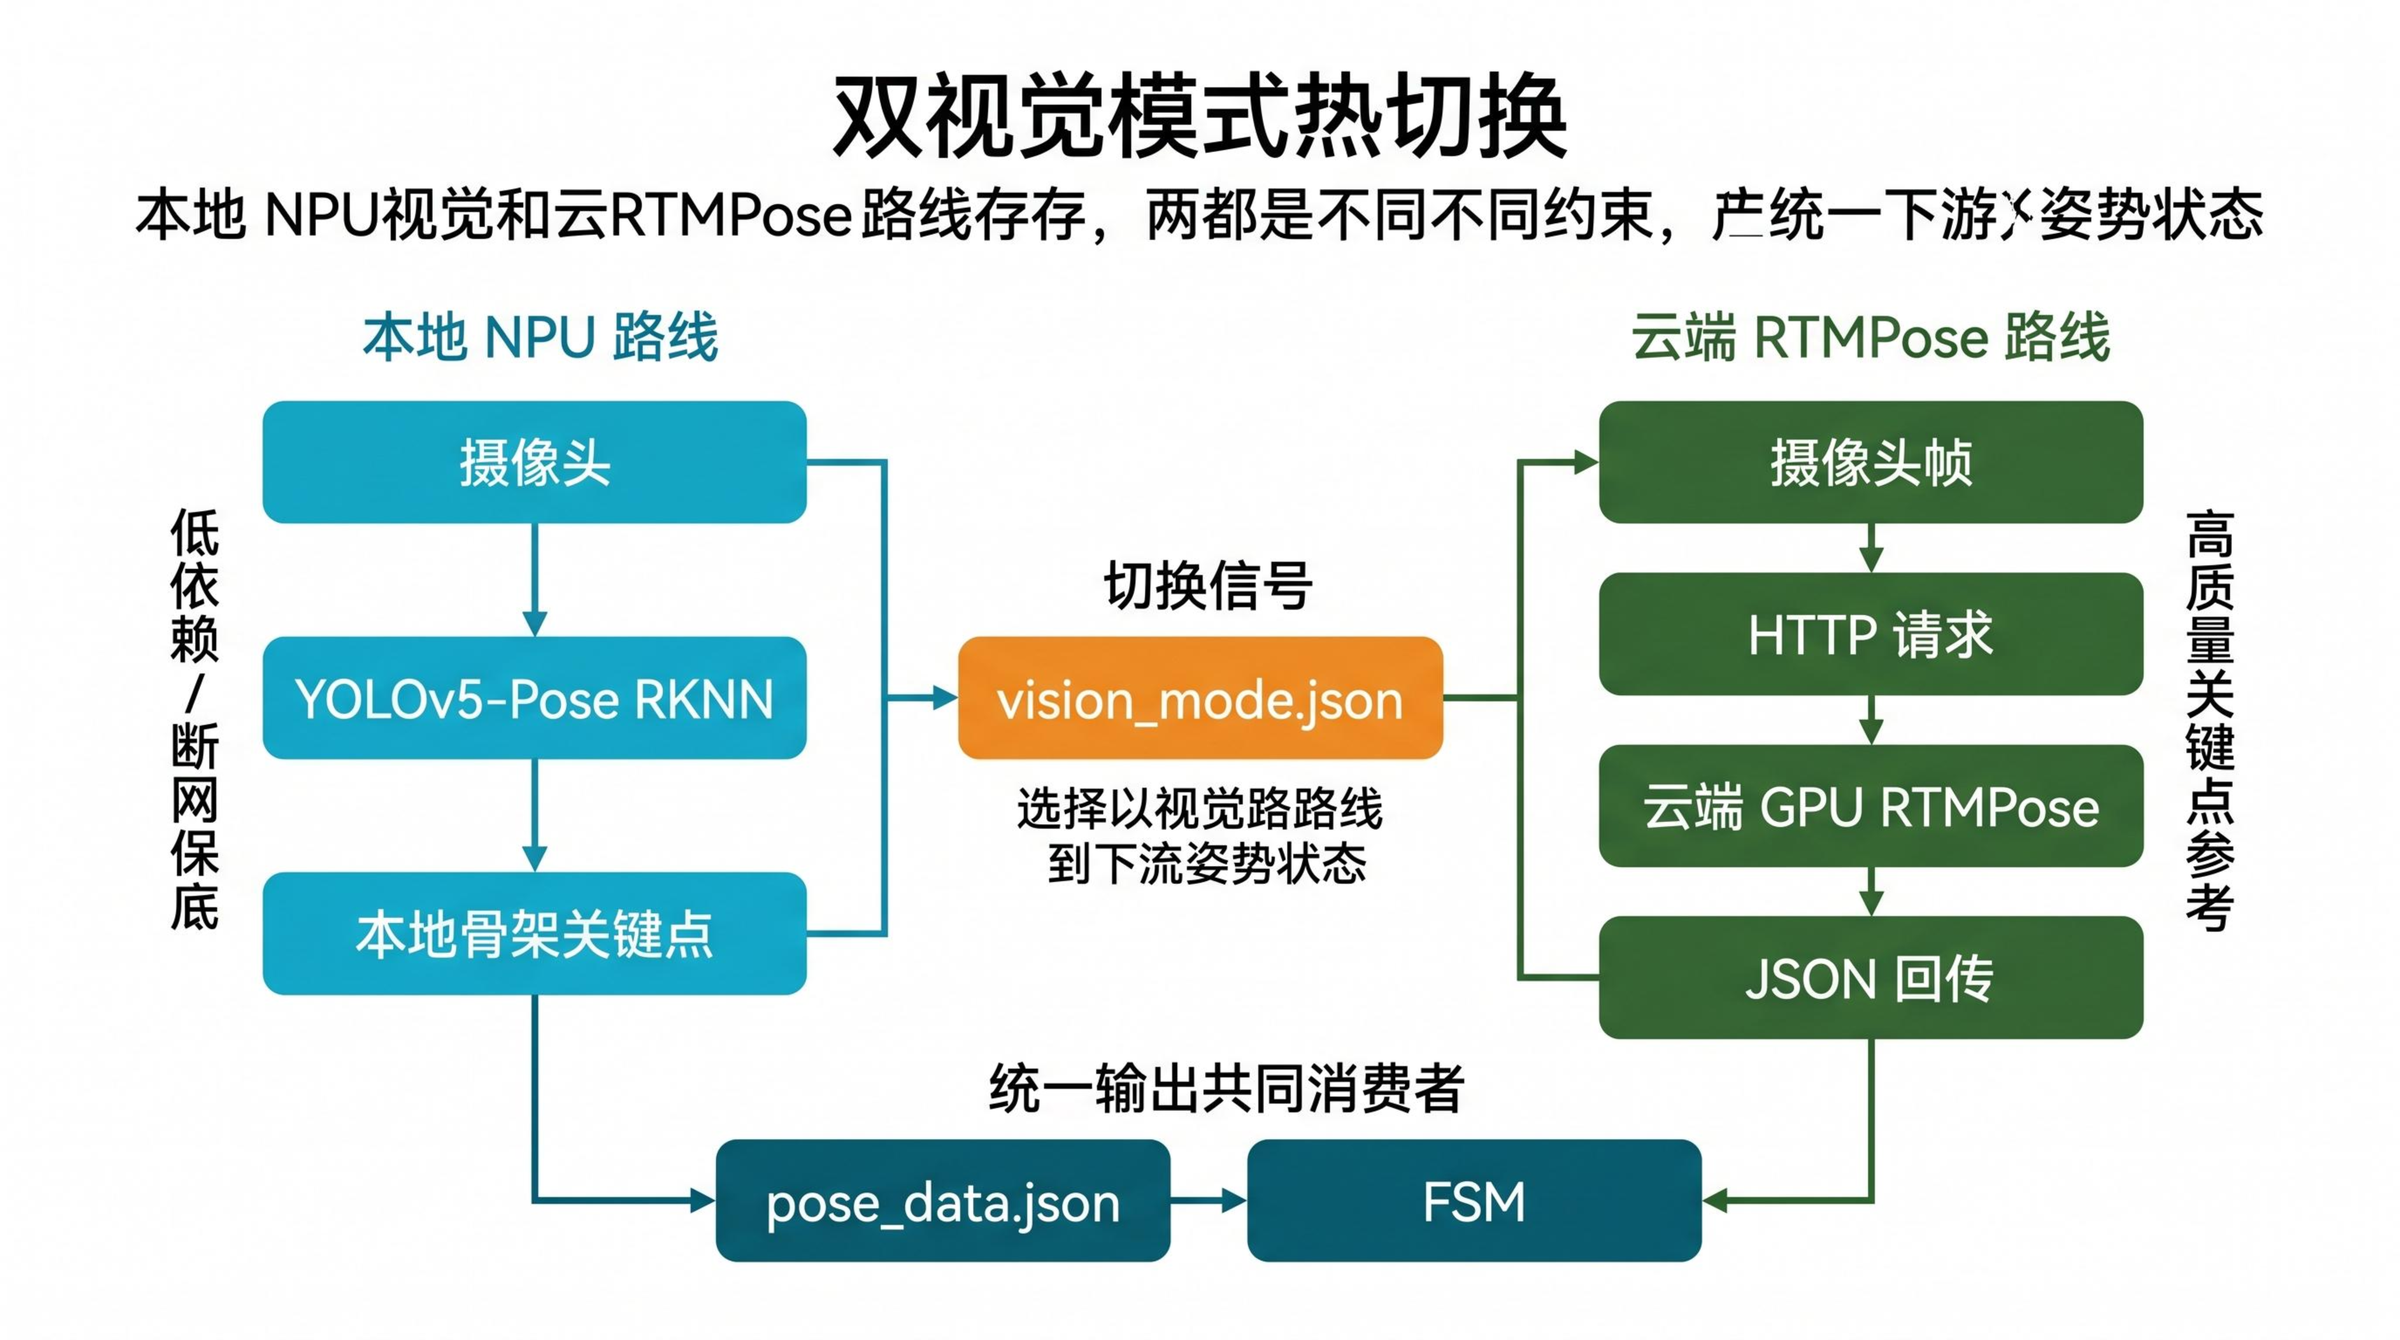
\includegraphics[width=0.92\textwidth]{figures/report/fig08.png}
    \caption{本地 NPU 与云端 RTMPose 并存的视觉路线。}
    \label{fig:dual-vision-switch}
\end{figure}

\subsubsection{肌电特征：MVC 归一化与个性化基准}

肌电特征不能直接用固定硬阈值解释。表面肌电的幅值会受到电极位置、皮肤
状态、个体肌肉基础、阻抗和动作方式影响。SENIAM 对表面肌电采集和电极
放置提出了规范建议 \cite{seniam}，EMG 幅值归一化也被长期讨论
\cite{burden2010,cede2020}。项目采用 MVC（Maximum Voluntary
Contraction）思路，让用户在训练前进行短时间最大发力，把该用户的峰值
作为个人基准。

在系统中，原始 RMS 经过个人 MVIC 峰值归一化后再进入特征窗口：
\[
    \%\mathrm{MVC}(t) = \frac{\mathrm{RMS}(t)}{\mathrm{MVIC}_{\mathrm{peak}}}\times 100\%.
\]
这是肌电幅值归一化的常见表达 \cite{burden2010,cede2020}。该数值不等于
严格的机械做功，更适合作为目标肌相对发力水平的工程近似。这样做的意义
在于，同一个固定阈值不会直接套在所有人身上，模型看到的是更接近"相对
发力水平"的输入。

\begin{figure}[htbp]
    \centering
    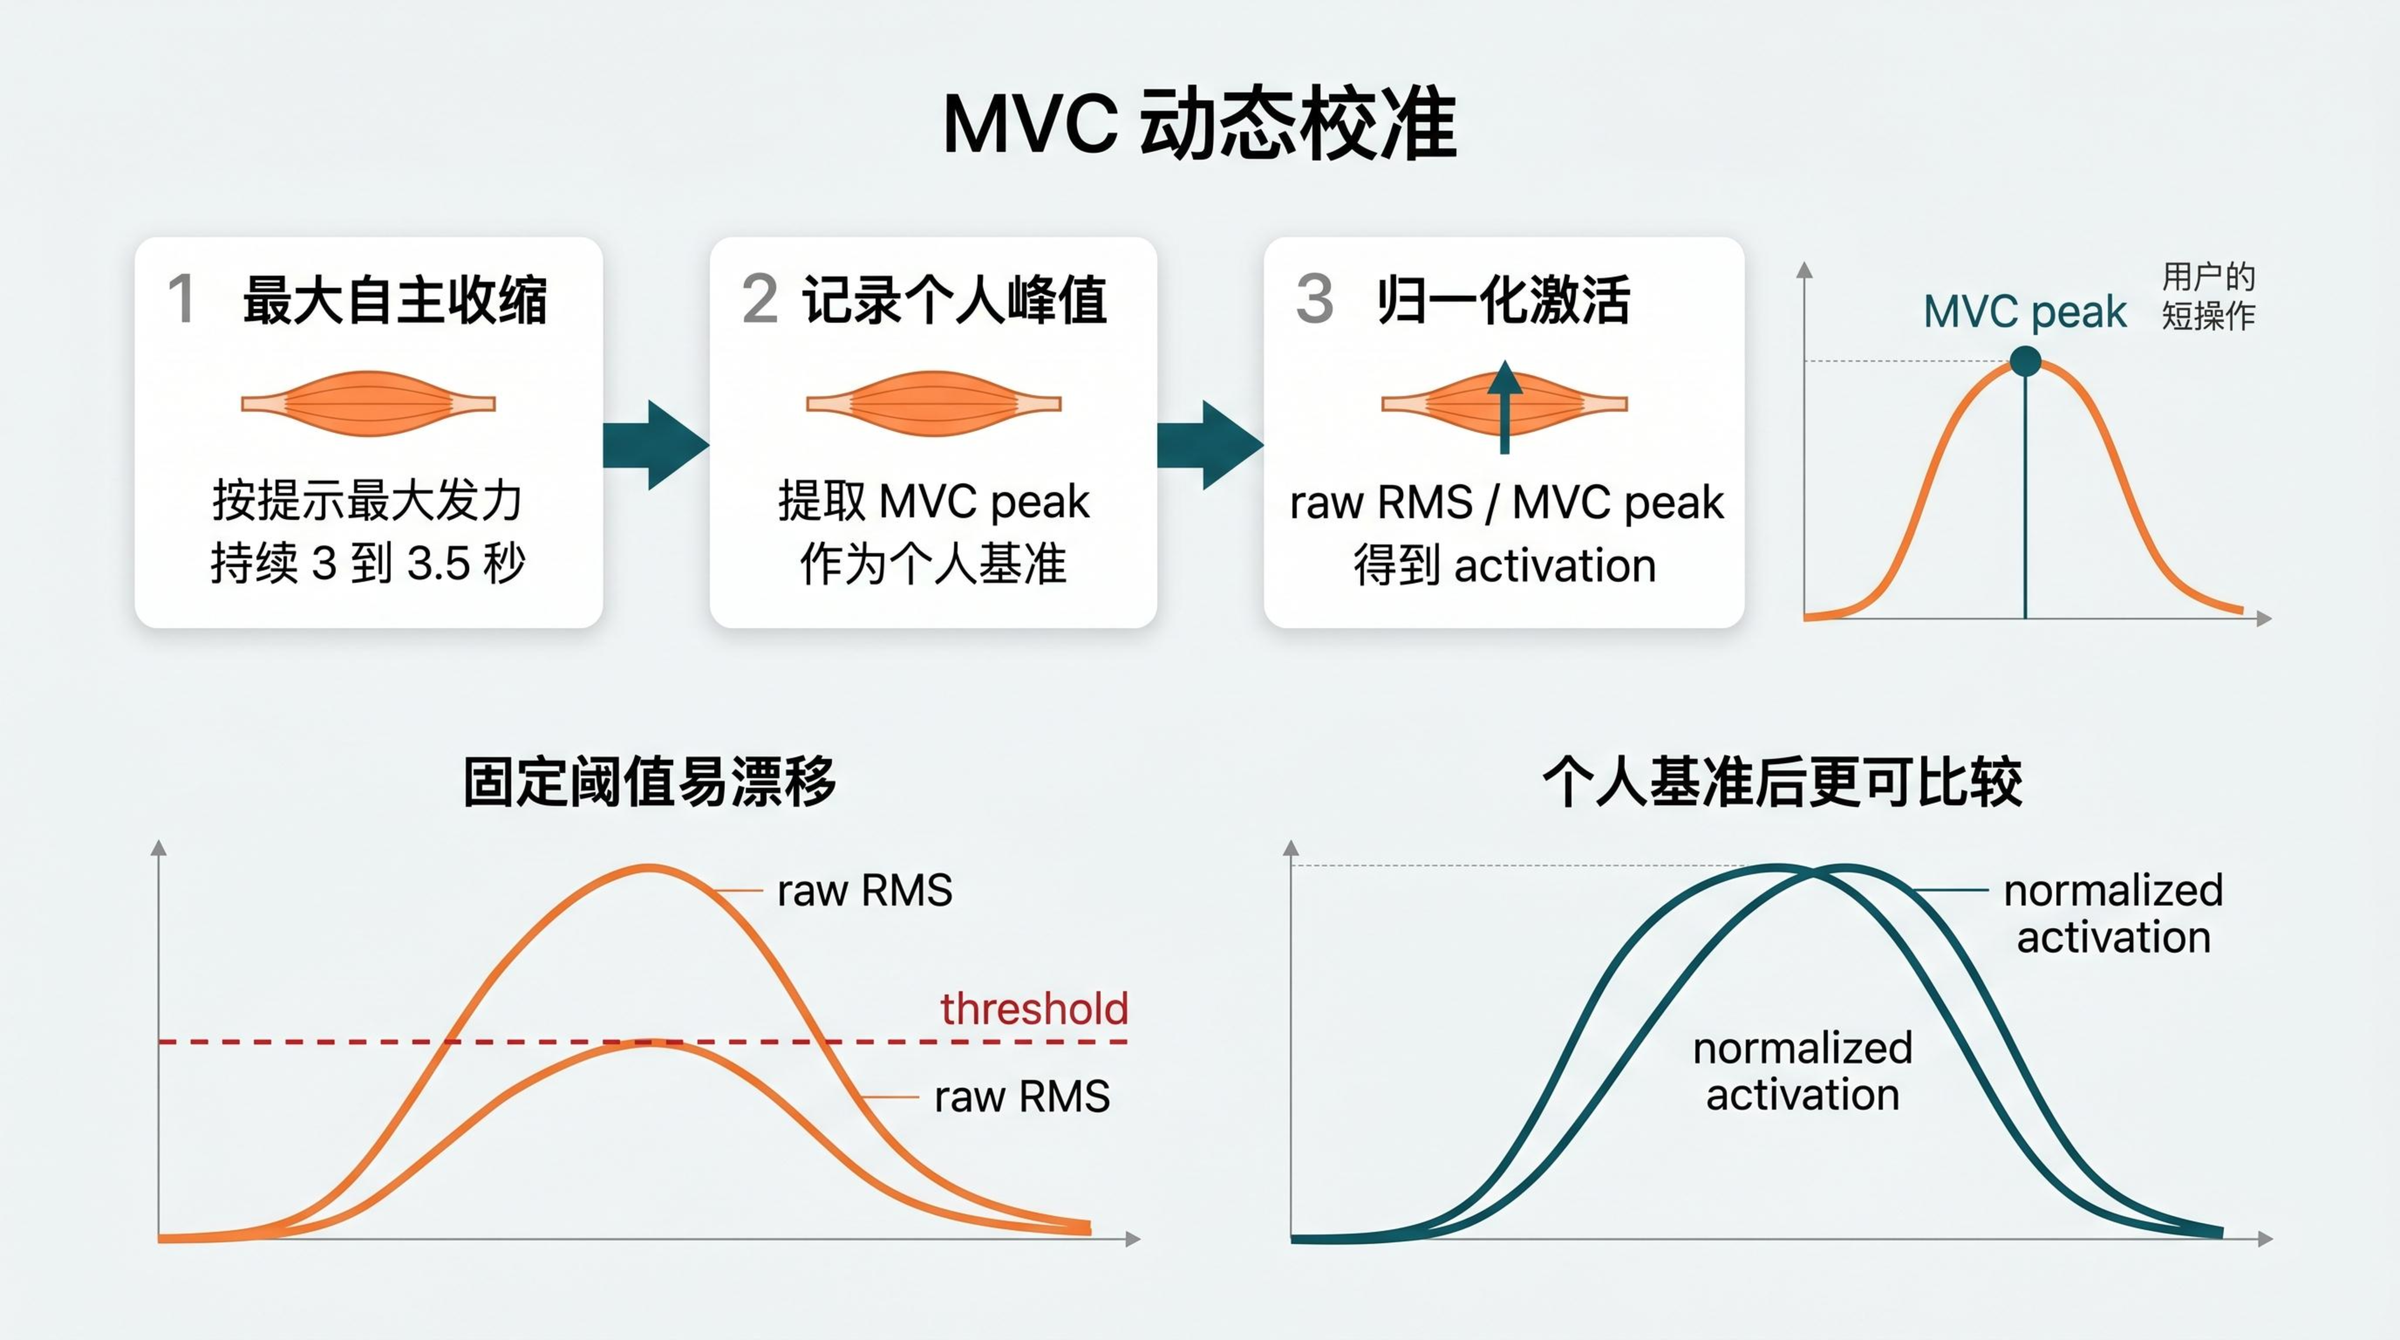
\includegraphics[width=0.9\textwidth]{figures/report/fig07.png}
    \caption{MVC 归一化校准流程示意。}
    \label{fig:mvc-calibration}
\end{figure}

\subsection{判断层：FSM 与 GRU 的分工}

感知层提供原始信号后，下一步要把它转化为可判断的动作质量。本节讨论
FSM 与 GRU 的分工，以及为什么选择 Mid-Fusion 而非端到端融合。

\subsubsection{从 if/else 到 GRU}

动作判断最终采用 FSM 与 GRU 分工，而不是只用规则或只用神经网络。FSM
负责动作阶段、上下行切换和次数统计，因为这部分与关节角度变化直接相关，
规则清楚、响应快，也方便调试。GRU 负责动作质量分类，因为代偿不是一个
单点阈值，而是一段动作周期里目标肌、代偿肌和动作相位之间的关系。

早期的 if/else 规则有明显优势：容易解释、容易快速跑通，也方便确认角度
阈值是否合理。但继续扩展到肌电后，规则很快变得脆弱。不同人、不同贴片
位置、不同动作幅度都会改变 RMS 分布；代偿动作也不一定表现为某一帧
突然越过阈值。门控循环单元（GRU）最早出现在 Cho 等人 2014 年提出的
RNN encoder-decoder 框架 \cite{gru} 中，它通过更新门与重置门在保留
历史状态和接收当前输入之间取得平衡，比朴素 RNN 更适合处理有限窗口
内的时序变化。本项目把最近一段 7D 特征窗口交给 CompensationGRU 做
标准、代偿和不标准三类判断。

\subsubsection{Mid-Fusion：在特征层融合}

多模态融合最终采用 Mid-Fusion \cite{baltrusaitis2018}。也就是说，视觉
和肌电不直接把原始序列硬拼进一个大模型，而是先转成低维、可解释的特征，
再进入轻量时序模型。视觉侧提取关节角度、角速度、角加速度和动作相位；
肌电侧提取目标肌 RMS、代偿肌 RMS，并结合对称性或阶段信息形成 7D 特征。
这个设计让模型输入更稳定，也让调试时能看懂每一列数据代表什么。

端到端融合在概念上更完整，但并不适合本项目当前条件。视觉关键点是低频
几何序列，肌电是更高频的生理信号；直接拼接会把时间对齐和噪声处理都推给
模型。板端算力、数据规模和现场调试也不支持一开始就采用复杂融合网络。
Mid-Fusion 把领域知识放在特征层，既保留了视觉和肌电的互补关系，也把
模型复杂度控制在当前板端和数据规模能够承受的范围内。

\begin{figure}[htbp]
    \centering
    \resizebox{0.96\textwidth}{!}{%
    \begin{tikzpicture}[
        node distance=0.9cm and 1.0cm,
        box/.style={draw, rounded corners=2pt, align=center, minimum width=2.8cm,
                    minimum height=0.8cm, font=\small},
        vision/.style={box, fill=cyan!9, draw=cyan!60!black},
        emg/.style={box, fill=orange!12, draw=orange!75!black},
        fuse/.style={box, fill=teal!10, draw=teal!70!black, minimum width=3.0cm},
        model/.style={box, fill=green!9, draw=green!55!black, minimum width=2.9cm},
        classout/.style={box, fill=gray!7, draw=gray!65, minimum width=1.7cm},
        arrow/.style={-{Latex[length=2mm]}, thick}
    ]
        \node[vision] (camera) {摄像头\\骨架关键点};
        \node[vision, right=of camera] (vfeat) {视觉特征\\关节角 / 角速度 / 相位};
        \node[emg, below=1.2cm of camera] (sensor) {sEMG 电极\\ESP32 UDP};
        \node[emg, right=of sensor] (efeat) {肌电特征\\RMS / MVC 归一化};
        \node[fuse, right=1.2cm of vfeat, yshift=-0.6cm] (window)
            {7D 特征窗口\\角度、角速度、角加速度\\目标肌 RMS、代偿肌 RMS\\对称性、动作相位};
        \node[model, right=1.0cm of window] (gru) {CompensationGRU\\轻量时序判断};
        \node[classout, right=0.9cm of gru, yshift=0.78cm, fill=green!12] (std) {标准};
        \node[classout, right=0.9cm of gru, fill=orange!12, draw=orange!70!black] (comp) {代偿};
        \node[classout, right=0.9cm of gru, yshift=-0.78cm, fill=red!8, draw=red!55!black] (bad) {不标准};

        \node[font=\bfseries\small, above=0.18cm of camera] {视觉流};
        \node[font=\bfseries\small, below=0.18cm of sensor] {肌电流};
        \node[font=\bfseries\small, above=0.18cm of window] {特征融合};
        \node[font=\bfseries\small, above=0.18cm of gru] {时序分类};

        \draw[arrow, cyan!70!black] (camera) -- (vfeat);
        \draw[arrow, orange!80!black] (sensor) -- (efeat);
        \draw[arrow, cyan!70!black] (vfeat) -- (window);
        \draw[arrow, orange!80!black] (efeat) -- (window);
        \draw[arrow, teal!75!black] (window) -- (gru);
        \draw[arrow, green!55!black] (gru) -- (std);
        \draw[arrow, orange!75!black] (gru) -- (comp);
        \draw[arrow, red!55!black] (gru) -- (bad);
    \end{tikzpicture}}
    \caption{Mid-Fusion 多模态特征融合路线。}
    \label{fig:mid-fusion}
\end{figure}

\subsection{交互层：LLM 与后台记录的边界}

判断结果最终要变成用户能看懂、系统能记住的反馈。本节说明 LLM 在前台
对话与后台总结之间的分工，以及训练数据的来源与边界。

\subsubsection{LLM 实时对话与后台总结分工}

大语言模型在系统里承担两类时间尺度不同的任务。前台 DeepSeek 主要用于
语音问答、训练提示和总结生成，要求上下文短、响应快；后台记录、数据库
和 OpenClaw 相关接口更适合保存训练历史、偏好变化和周期性总结，允许
更长的上下文和更慢的处理。项目把二者分开，是为了避免实时反馈被长期
分析拖慢，也避免后台记录直接影响训练主链路。

当前系统已经能展示知识库命中、云端记忆、数据库表和调试入口。它们的
价值在于让训练数据和调试证据不再散落在黑盒里。长期记忆、用户画像和
周期性计划属于后续扩展方向；在当前报告中，它们作为可维护性和可演进性
的接口来描述。

\subsubsection{数据来源与训练边界}

多模态健身数据集是项目中的现实难点。公开数据可以提供动作周期、肌电
模式和姿态估计的先验，但很难完全匹配本项目的硬件、贴片位置、动作定义
和训练场景。项目因此采用公开数据、本地采集、模拟数据和数据增强结合
的路线：公开数据中，EMAHA-DB6 提供较完整的多通道 sEMG 动作样本，
MIA 数据集提供肌电与运动学同步标注，Mendeley 公开的 sEMG 弯举数据集
提供个体差异的参考分布；这些公开样本主要用于建立特征分布的先验，本地
采集用于贴近本项目的 ESP32 + 4 通道贴片硬件域，增强数据则在公开与
本地样本上进一步扩大训练过程中的扰动范围（噪声注入、随机平移、贴片
偏移模拟等）\cite{lara2013}。

增强数据和本地数据可以帮助模型学习当前任务中的区分信号，但训练策略
仅在当前数据规模下适用，不直接外推到跨用户、跨环境的稳定泛化。

\subsection*{本章小结}
\addcontentsline{toc}{subsection}{本章小结}

上述选择共同服务于一个目标：让系统在边缘设备上可运行、可调试，并能
围绕真实训练流程持续扩展。它们不是单点技术堆叠，而是围绕真实训练
流程不断收敛出来的工程取舍。

\begin{table}[htbp]
\centering
\small
\begin{tabular}{@{}>{\raggedright\arraybackslash}p{0.23\textwidth}
                >{\raggedright\arraybackslash}p{0.28\textwidth}
                >{\raggedright\arraybackslash}p{0.37\textwidth}@{}}
\toprule
\textbf{岔路} & \textbf{最后选择} & \textbf{原因} \\
\midrule
视觉模型 & YOLOv5-Pose + RTMPose 双路线 & 本地路线降低网络依赖，云端路线
提供关键点质量参考，通过状态文件切换。 \\
动作判断 & FSM 计数 + GRU 分类 & 计数是几何问题，质量判断是时序和肌电
共同作用的问题。 \\
多模态融合 & Mid-Fusion & 端到端融合对板端算力和数据规模要求过高，
先降维到可解释特征更稳。 \\
肌电基准 & MVC 归一化 & 用个人峰值减少固定阈值在不同个体之间的漂移。 \\
LLM 接入 & 实时对话 + 后台记录接口 & 即时反馈和长期整理的时间尺度不同，
拆开后边界更清楚。 \\
\bottomrule
\end{tabular}
\caption{项目中的关键技术取舍}
\label{tab:decisions}
\end{table}
